\documentclass[hidelinks,12pt]{article}
\usepackage[left=0.25cm,top=1cm,right=0.25cm,bottom=1cm]{geometry}
%\usepackage[landscape]{geometry}
\textwidth = 20cm
\hoffset = -1cm
\usepackage[utf8]{inputenc}
\usepackage[spanish,es-tabla, es-lcroman]{babel}
\usepackage[autostyle,spanish=mexican]{csquotes}
\usepackage[tbtags]{amsmath}
\usepackage{nccmath}
\usepackage{amsthm}
\usepackage{amssymb}
\usepackage{mathrsfs}
\usepackage{graphicx}
\usepackage{subfig}
\usepackage{caption}
%\usepackage{subcaption}
\usepackage{standalone}
\usepackage[outdir=./Imagenes/]{epstopdf}
\usepackage{siunitx}
\usepackage{physics}
\usepackage{color}
\usepackage{float}
\usepackage{hyperref}
\usepackage{multicol}
\usepackage{multirow}
%\usepackage{milista}
\usepackage{anyfontsize}
\usepackage{anysize}
%\usepackage{enumerate}
\usepackage[shortlabels]{enumitem}
\usepackage{capt-of}
\usepackage{bm}
\usepackage{mdframed}
\usepackage{relsize}
\usepackage{placeins}
\usepackage{empheq}
\usepackage{cancel}
\usepackage{pdfpages}
\usepackage{wrapfig}
\usepackage[flushleft]{threeparttable}
\usepackage{makecell}
\usepackage{fancyhdr}
\usepackage{tikz}
\usepackage{bigints}
\usepackage{menukeys}
\usepackage{tcolorbox}
\tcbuselibrary{breakable}
\usepackage{scalerel}
\usepackage{pgfplots}
\usepackage{pdflscape}
\pgfplotsset{compat=1.16}
\spanishdecimal{.}
\renewcommand{\baselinestretch}{1.5} 
\renewcommand\labelenumii{\theenumi.{\arabic{enumii}})}

\newcommand{\python}{\texttt{python}}
\newcommand{\textoazul}[1]{\textcolor{blue}{#1}}
\newcommand{\azulfuerte}[1]{\textcolor{blue}{\textbf{#1}}}
\newcommand{\funcionazul}[1]{\textcolor{blue}{\textbf{\texttt{#1}}}}

\newcommand{\pderivada}[1]{\ensuremath{{#1}^{\prime}}}
\newcommand{\sderivada}[1]{\ensuremath{{#1}^{\prime \prime}}}
\newcommand{\tderivada}[1]{\ensuremath{{#1}^{\prime \prime \prime}}}
\newcommand{\nderivada}[2]{\ensuremath{{#1}^{(#2)}}}


\newtheorem{defi}{{\it Definición}}[section]
\newtheorem{teo}{{\it Teorema}}[section]
\newtheorem{ejemplo}{{\it Ejemplo}}[section]
\newtheorem{propiedad}{{\it Propiedad}}[section]
\newtheorem{lema}{{\it Lema}}[section]
\newtheorem{cor}{Corolario}
\newtheorem{ejer}{Ejercicio}[section]

\newlist{milista}{enumerate}{2}
\setlist[milista,1]{label=\arabic*)}
\setlist[milista,2]{label=\arabic{milistai}.\arabic*)}
\newlength{\depthofsumsign}
\setlength{\depthofsumsign}{\depthof{$\sum$}}
\newcommand{\nsum}[1][1.4]{% only for \displaystyle
    \mathop{%
        \raisebox
            {-#1\depthofsumsign+1\depthofsumsign}
            {\scalebox
                {#1}
                {$\displaystyle\sum$}%
            }
    }
}
\def\scaleint#1{\vcenter{\hbox{\scaleto[3ex]{\displaystyle\int}{#1}}}}
\def\scaleoint#1{\vcenter{\hbox{\scaleto[3ex]{\displaystyle\oint}{#1}}}}
\def\scaleiiint#1{\vcenter{\hbox{\scaleto[3ex]{\displaystyle\iiint}{#1}}}}
\def\bs{\mkern-12mu}

\newcommand{\Cancel}[2][black]{{\color{#1}\cancel{\color{black}#2}}}


\usepackage{minted}

\author{M. en C. Gustavo Contreras Mayén. \texttt{gux7avo@ciencias.unam.mx}}
\title{Evaluación del Examen Final \\ {\large Curso Física Computacional}}
\date{ }
\begin{document}

\maketitle
\fontsize{14}{14}\selectfont

\section{Problema 1.}

\begin{enumerate}
\item Al momento de ejecutar el código, marca un error por que no está la correspondiente referencia a $3$ módulos, aunque los dejaste en una carpeta, en el código de tu ejercicio debería de indicarse.
\begin{figure}[H]
    \centering
    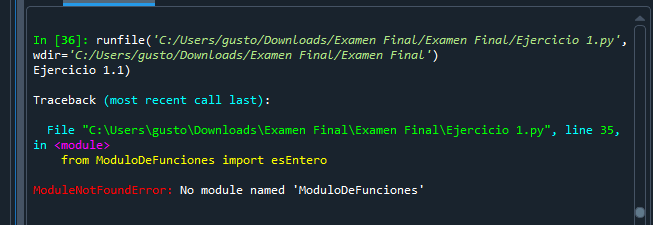
\includegraphics[scale=0.8]{Evidencia_Antonio_01.png}
\end{figure}
\begin{figure}[H]
    \centering
    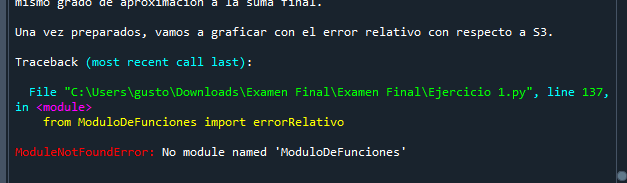
\includegraphics[scale=0.8]{Evidencia_Antonio_02.png}
\end{figure}
\begin{figure}[H]
    \centering
    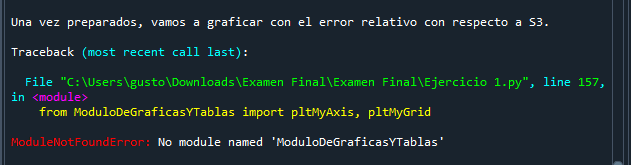
\includegraphics[scale=0.8]{Evidencia_Antonio_03.png}
\end{figure}
Esto es independiente del entorno de desarrollo que utilices, en la siguiente imagen, desde una terminal se ejecuta python y el error se hace presente.
\begin{figure}[H]
    \centering
    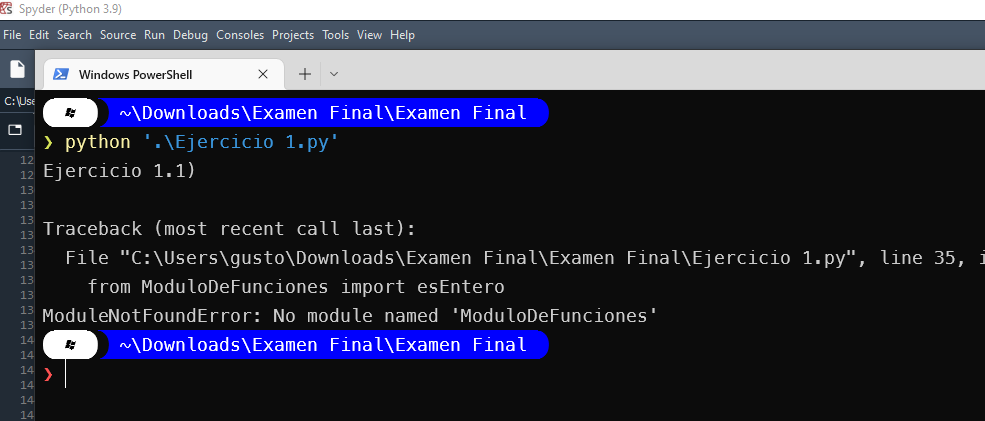
\includegraphics[scale=0.5]{Evidencia_Antonio_04.png}
\end{figure}
Este tipo de situaciones se aclara en la rúbrica de evaluación que deben de evitarse, es lo que te descuenta puntaje.
\item Es recomendable que separes las gráficas para tener una mayor claridad con respecto al resultado que presentas, en tu caso, se superponen los resultados, la interpretación que das es congruente, pero la gráfica aunque la hiciste bien, al dejar el error de ambos procedimientos para la suma, ya no deja ver su tendencia.
\item \textbf{Calificación: 0.7 puntos}
\end{enumerate}

\section{Problema 2.}

\begin{enumerate}
\item Nuevamente hay problemas para las llamadas a las funciones.
\begin{figure}[H]
    \centering
    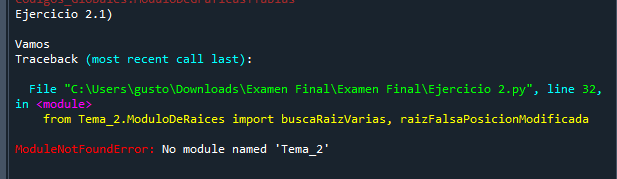
\includegraphics[scale=0.8]{Evidencia_Antonio_05.png}
\end{figure}
Llama la atención que dentro de una carpeta global, tengas otras carpetas con módulos específicos, la idea es buena, pero la ejecución de tu código debe de ser también sin contratiempos.
\begin{figure}[H]
    \centering
    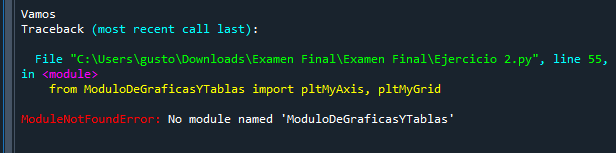
\includegraphics[scale=0.8]{Evidencia_Antonio_06.png}
\end{figure}
\item Creas la función para obtener una raíz con el método de la falsa posición modificada, recomiendo que comentas más tu código, a modo de evidencia de que la función hace lo que se espera, no digo que no lo haga, pero ayuda mucho cuando hay comentarios al respecto.
\item La parte de las gráficas para cada inciso es correcta.
\item \textbf{Calificación: 0.8 puntos.}
\end{enumerate}

\section{Problema 3.}

\begin{enumerate}
\item Con el antecedente de los primeros problemas, hay errores para las llamadas a las funciones.
\item No queda claro el por qué tienes la siguiente función:
\begin{minted}{python}
def g_E(u):
    if u == 0:
        ylim = np.inf
    else:
        ylim = 1/u

    def f(x): return x**4*np.exp(x) /(np.exp(x)-1)**2
    I = quad(f, 0, ylim)[0]
    value = u**3* I 
        
    return value
\end{minted}
El condicional no explica propiamente lo que quieres hacer, es cierto que se tendría que haber estudiado previamente la función a integrar, ver si es finita cuando $x  \to 0$.
\item Ahora bien, aunque mencionas que \enquote{Vamos a usar scipy cómo método de comparación}, la solución que presentas es con esa función. Se indicó que todas las funciones de python se podrían utilizar con el fin de corroborar sus resultados, no para resolver el problema. Tenías varias técnicas de integración con códigos que revisamos en clase.
\item El problema devuelve la solución correcta, pero no se considera por que no utilizaste lo que se trabajó en el curso.
\item \textbf{Calificación: 0 puntos.}
\end{enumerate}

\section{Problema 4.}

\begin{enumerate}
\item En este ejercicio vuelves a utilizar una función de \texttt{scipy} para presentar la solución. Se esperaba que implementases un código con lo que se trabajó en clase.
\item \textbf{Calificación: 0 puntos.}
\end{enumerate}

\section{Problema 5.}

\begin{enumerate}
\item Se encuentra un error de ejecución por que no ubica los módulos necesarios.
\item Te recomiendo que utilices una sola vez la referencia de los módulos, ya que para cada celda, haces nuevamente la llamada, no es necesario ya que se carga de manera general, y la ejecución de cada celda ocupa esa referencia.
\item ¿Por qué utilizaste RK4?
\item \textbf{Calificación: 0.9 puntos.}
\end{enumerate}

\section{Problema 6.}

\begin{enumerate}
\item En conjunto con el notebook de Jupyter resuelves bien el ejercicio.
\item Este tipo de solución es el que se espera en un examen, te aplicaste bien en el ejercicio.
\item \textbf{Calificación: 1 punto.}
\end{enumerate}

\section{Problema 7.}

\begin{enumerate}
\item El enunciado del problema inicialmente pide que con el método de diferencias finitas se desarrolle el sistema de ecuaciones algebraicas $\vb{A \, x} = \vb{b}$, que si bien comienzas, no quedan expresadas las matrices que luego vas a ocupar.
\item No aclaras quiénes son $\alpha$ y $\beta$ a partir de la CDF.
\item La gráfica de la solución del inciso a) es correcta.
\item En la gráfica de la solución para el inciso b) hay una diferencia, que deberías de haber identificado en el cumplimiento de la CDF de la ED.
\begin{figure}[H]
    \centering
    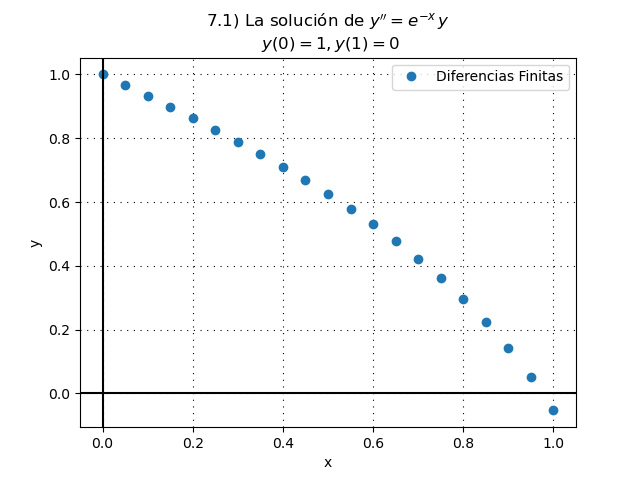
\includegraphics[scale=0.7]{Evidencia_Antonio_07.png}
    \caption{Tu solución que no satisface la CDF $y(1) = 0$}
\end{figure}
Cuando la solución esperada es:
\begin{figure}[H]
    \centering
    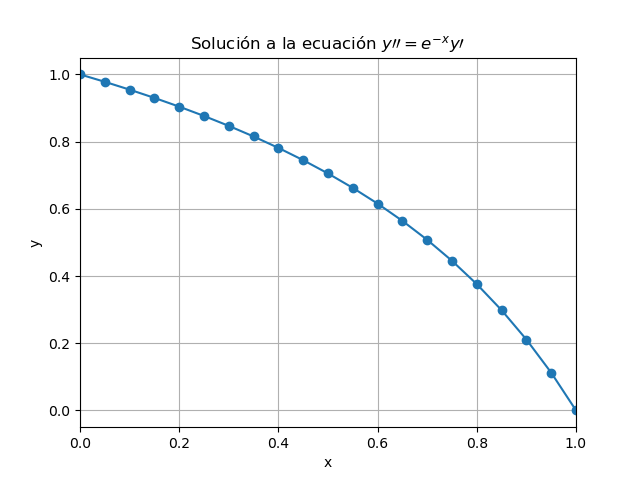
\includegraphics[scale=0.7]{Evidencia_Antonio_08.png}
    \caption{En esta solución se satisface la CDF $y(1) = 0$}
\end{figure}
\item \textbf{Calificación: 0.7 puntos.}
\end{enumerate}

\section{Problema 8.}

\begin{enumerate}
\item Error en la llamada a los módulos.
\item En ambos incisos planteas un intervalo superior de integración razonable, aunque $10$ sigue siendo un valor alto, pero te funciona.
\item Bien por plantear el método que se trabajó en clase para generar los valores aleatorios.
\item Presentas gráficas que muestran la tendencia del error relativo para la aproximación de la integral, que es una parte necesaria de la solución.
\item Se esperaba que mostrases las gráficas de puntos aleatorios por debajo de la curva y por encima de ella, para diferentes valores de $n$.
\item \textbf{Calificación: 0.9 puntos.}
\end{enumerate}

\section{Problema 9.}

\begin{enumerate}
\item Error en las llamadas a los módulos.
\item El problema no presenta la solución completa.
\item Faltó trabajar más el abordaje para el mismo, que buena ayuda proporciona en la implementación del código. No tienes un círculo unitario, tienes un hemisferio de radio $1$.
\begin{figure}
    \centering
    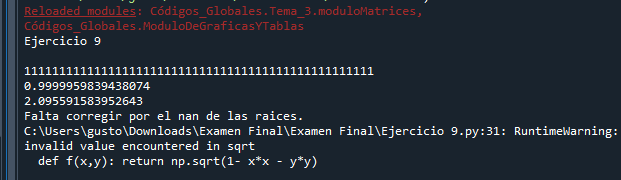
\includegraphics[scale=0.8]{Evidencia_Antonio_09.png}
\end{figure}
\item \textbf{Calificación: 0 puntos.}
\end{enumerate}





\end{document}